%\documentclass{beamer}
\documentclass[brown]{beamer}
\usepackage{beamerthemesplit}
%\usepackage{beamerthemeshadow}
%\usetheme{default} 

\usepackage{amsfonts}
\usepackage{amssymb}
\usepackage{amsmath}
\usepackage{dsfont}
\usepackage{graphicx}
\usepackage{varioref}

\usepackage{color}
\definecolor{yellow}{rgb}{1,1,0}
\definecolor{black}{rgb}{0,0,0}
\definecolor{ltcyan}{rgb}{.75,1,1}
\definecolor{blue}{rgb}{0,0,1}
\definecolor{red}{rgb}{1,0,0}
\definecolor{darkred}{rgb}{0.5,0,0}
\definecolor{darkgreen}{rgb}{0,0.5,0}

\usepackage{listings}
\lstloadlanguages{C,C++}
\lstset{fontadjust=false,basicstyle=\small\ttfamily}
\lstset{language=C}
\lstdefinelanguage{Dax}{
  morekeywords={WorkMapField,WorkMapCell,Cell,Field,FieldCell,FieldPoint,FieldCoordinates,Scalar,Vector3,Vector4},
  morekeywords={[2]dax,exec,comp},
  morekeywords={[3]DAX_WORKLET,DAX_IN,DAX_OUT}
}
\lstset{
  keywordstyle=\color{blue},
  keywordstyle=[2]\color{darkred},
  keywordstyle=[3]\color{darkgreen}
}

\newcommand*{\textC}[1]{\texttt{#1}}

\title{\textbf{Dax Toolkit}: \\
  A Proposed Framework for Data Analysis and Visualization \\
  at Extreme Scale}

\author{\small
  Kenneth Moreland {\tiny Sandia National Laboratories} \\
  \textbf{Utkarsh Ayachit} {\tiny Kitware, Inc. } \\
  Berk Geveci {\tiny Kitware, Inc. }\\
  Kwan-Liu Ma {\tiny University of California at Davis}
}
%\author{Kenneth Moreland \\
%\textbf{Utkarsh Ayachit} \\
%Berk Geveci\\
%Kwan-Liu Ma}
\date {October 24, 2011}

\setbeamertemplate{footline}{}
\beamertemplatenavigationsymbolsempty

\begin{document}
\frame{\titlepage}

%\section{Introduction}
\frame
{
  %\frametitle{In this talk...}
  \begin{beamerboxesrounded}{Dax Toolkit}
  A new visualization framework designed to exhibit the pervasive parallelism
    necessary for exascale machines.
  \end{beamerboxesrounded}
}

\section{Motivation}
\subsection{Background}

\frame
{
  \frametitle{Visualization Pipeline}
  % Talk about the visualization pipeline.
  \begin{figure}
  \centering
  \includegraphics[width=.8\textwidth]{images/SimplePipeline.pdf}
  \end{figure}
}

\frame
{
  \frametitle{Parallel Visualization Pipeline}
  %Talk about how VTK/ParaView/VisIt deal with parallelism.
  \begin{figure}
  \centering
  \includegraphics[width=.8\textwidth]{images/ParallelVisPipeline.pdf}
  \end{figure}
}


\frame
{
  \frametitle{Petascale To Exascale\footnote[1]{Estimates consolidated from International
  Exascale Software Project Roadmap and the DOE Exascale Initiative Roadmap.}}
  \renewcommand{\arraystretch}{1.5}
  \begin{table}[htbp]
    \centering
    \begin{tabular}{l|l|l|l}
      & Jaguar -- XT5 & Exascale & Increase \\
      \hline
      Cores & 224,256
      & 100 million -- 1 billion
      & 400 -- 5,000$\times$ \\
      Threads & 224,256 way
      & 1 -- 10 billion way
      & 4,000 -- 50,000$\times$ \\
      Memory & 300 Terabytes
      & 10 -- 128  Petabytes
      & 30 -- 500$\times$
    \end{tabular}
  \end{table}
}

\subsection{Our Approach}
\frame
{
  \frametitle{Revisiting the Filter}
  \begin{figure}
  \centering
  \includegraphics[width=0.5\textwidth]{images/SingleElementFilter.pdf}
  \end{figure}
}

\frame
{
  \begin{center}
  function (\emph{in}, \emph{out})
  \end{center}
}

\frame
{
  \begin{center}
  \includegraphics[width=0.3\textwidth]{images/worklet.pdf}
  \end{center}
}

\frame
{
  \begin{center}
  \includegraphics[width=\textwidth]{images/many_worklets.pdf}
  \end{center}
}

\subsection{Related Work}
\frame
{
  \frametitle{Existing Approaches}
  Summarize existing approaches and contrast with our proposal.
}

\section{Dax Toolkit}

\frame
{
  \frametitle{System Overview}
  Why GPU? Why CUDA?
}

\frame
{
  \frametitle{Data Model}
  Describe dax::exec::Work and dax::exec::Field.
}

\frame
{
  \frametitle{Dax Programming Environments}
  \begin{figure}[htbp]
    \centering
    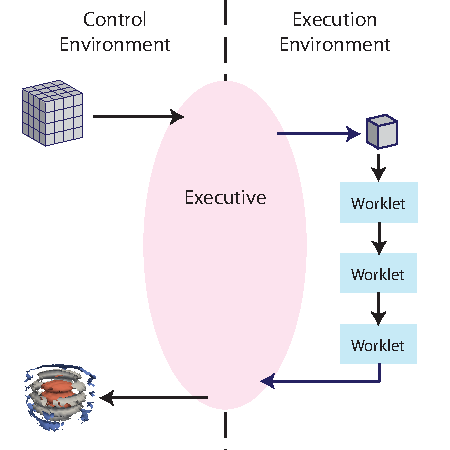
\includegraphics{images/DaxDiagram}
  \end{figure}
}

\subsection{Execution Environment}
\frame
{
  \frametitle{Execution Environment}
  One or two sample worklets describing how the execution environment works.
}

\subsection{Control Environment}
\frame
{
  \frametitle{Control Environment}
  Example of how the control environment looks.
}

\section{Results}

\frame
{
  \frametitle{Code Comparison}
  Compare cell-derivatives code.
}

\frame
{
  \frametitle{Performance Comparison}
  \begin{table}[htbp]
    \centering
    \label{tab:Results}
    %\vspace{6pt}
    \begin{tabular}{llrrr}
      \qquad & Mesh Size & VTK Time & Dax Time & Speedup \\
      \hline
      \multicolumn{5}{l}{Elevation $\rightarrow$ Gradient} \\
      %% & $144^3$ & 2.75 s & 0.02 (0.03) s & 138 (92) \\
      %% & $256^3$ &  15.52 s & 0.11 (0.19) s & 141 (82) \\
      %% & $512^3$ &  125.75 s & 0.89 (1.57) s &  141 (80) \\
      & $144^3$ & 2.75 s & 0.013 (0.024) s & 210 (114) \\
      & $256^3$ &  15.52 s & 0.074 (0.135) s & 210 (115) \\
      & $512^3$ &  125.75 s & 0.589 (1.076) s &  213 (117) \\
      \multicolumn{5}{l}{Elevation $\rightarrow$ Sine $\rightarrow$ Square $\rightarrow$ Cosine} \\
      & $144^3$ & 2.32 s & 0.002 (0.006) s &  1169 (386) \\
      & $256^3$ &  12.99 s & 0.013 (0.034) s & 999 (382) \\
      & $512^3$ & 103.88 s & 0.110 (0.276) s &  944 (376) \\
    \end{tabular} 
  \end{table}
  {Performance comparison between Dax toolkit and VTK. Values in
  parentheses show the corresponding values with data transfer times
  included}.
}

\frame
{
  \frametitle{Ongoing Work}
  Summarize the challenges ahead and some of the ongoing work.
}

\frame
{
  \frametitle{Conclusion}
  Dax Toolkit
}

\frame
{
  \frametitle{Acknowledgements}
  This work was supported in full by the DOE Office of Science, Advanced
  Scientific Computing Research, under award number 10-014707, program manager
  Lucy Nowell.
}

\end{document}
